\documentclass[a4page, 11pt]{article}

\usepackage{graphicx}
\usepackage{hyperref} %clickable stuffs
\usepackage{mathtools}
\usepackage[margin=0.65in]{geometry}
\usepackage[utf8]{inputenc}
\usepackage[english]{babel}
\usepackage[autostyle]{csquotes}
\MakeOuterQuote{"} %almost there, i removed `` everywhere to make it work better! D.
\usepackage{enumitem}
\usepackage[backend=biber]{biblatex} % pls uncomment me (Maurino's english style) but... what's the actual scope here?
%It was to print the bibliography, just to be give credit to the author of the original content but I guess we could leave it in a separate file biblio and print it here

\addbibresource{biblio.bib}
%Aggiungere alla biblio anche gli autori degli appunti dell'anno scorso (se sapete i nomi)


\graphicspath{ {./img/} }

\title{Data Management}
\author{}
\date{}

\begin{document}

\maketitle
%\tableofcontents %maybe would be nice to add?
%Some one commented it (MoMo) so I thought it was not necessary

\section{Data Modelling}
Il data modelling è uno strumento per descrivere parte del mondo reale che ci permette di:
\begin{itemize}[noitemsep]
\item Immagazzinare dati (write data)
\item Interrogare i dati (read data)
\end{itemize}
Un data model è composto prima di tutto da un modello concettuale (teoria) e poi da un linguaggio (anche grafico a volte) per descrivere e interrogare i dati. Un data model è sempre disponibile in un databasse management system che supporta la semantica del modello. Alcune delle caratteristiche più importanti di un data model sono:
\begin{itemize}[noitemsep]
\item Machine readability
\item Expressive power
\item Semplicità? Flessibilità? Standardizzazione?
\end{itemize}
Il data model più famoso  e conosciuto è il modello relazionale.
\subsection{Relational model}

Aspetti positivi :

\begin{enumerate}[noitemsep]
	 
	\item
	Molto rigido come regole.
	\item
	Il RDBMS sfrutta le proprietà ACID :
	\begin{itemize}
		
		\item
		A : Atomicity : serve affinché l'operazione o avviene su tutti i dati o non avviene, ad esempio se vi è un aggiornamento nei dati questo aiuta affinché i dati non vengano aggiornati solo parzialmente.
		\item
		C : Consistency : I dati o il nuovo dato che viene aggiunto rispetta lo schema prestabilito. E se si viola la consistenza con un'operazione tutta l'operazione fallisce.
		\item
		I : Isolation : gestisce come l'integrità delle transazioni sono viste dall'utente. Inoltre garantisce che durante un'operazione (query) non vengano svolte altre operazioni, e che lo stato del database venga modificato solo prima della fine della query.
		\item
		D : Durability : garantisce che una transazione effettuata sopravvivrà per sempre, anche se il sistema crasha. Dovuto grazie ai server di
		backup e log files.
	\end{itemize}
\end{enumerate}
Il RDBMS esiste già da 35 anni quindi è ben sviluppato e molto conosciuto, molti dati sono ancora salvati in questo formato ed è efficace ancora per molte operazioni. Gli aspetti limitanti sono:

\begin{enumerate}[noitemsep]
	 
	\item
	un attributo può avere solo un valore.
	\item
	non è compatibile con molti linguaggi moderni.
	\item
	molto rigido come linguaggio
	\item
	non accetta i loop.
	\item
	Difficile modificare le tabelle.
	\item
	La performance.
\end{enumerate}
Nei RDBMS la performance (inteso come velocità) dipende da vari fattori:
\begin{itemize}[noitemsep]
	 
	\item
	Numero delle righe
	\item
	Tipo di operazione
	\item
	Algoritmo scelto
	\item
	La struttura dati scelta
\end{itemize}

Per Scaling Up intendiamo potenziare le macchine, mentre per Scaling out intendiamo aggiungere macchine, per i RDBMS è più facile Scale up che Scale out. 
Il costo è un altro dei problemi, installare il software richiede un costo molto alto e hardware molto complesso.
Inoltre se continuiamo a aggiungere server (scaling out) il prezzo dell'Hardware aumenta esponenzialmente mentre il guadagno complessivo sul tempo di risposta scende asintoticamente.
\newline
\subsection{NoSQL}
Di fronte a questi svantaggi sorge una nuova "tecnologia": i NoSQL(Not Only SQL).
Le proprietà dei NoSQL sono:

\begin{enumerate}[noitemsep]
	 
	\item
	Non hanno nessuno schema o modello prefissato
	\begin{itemize}
		
		\item
		A differenza dei modelli SQL nei quali bisogna prima definire il modello, nel caso NoSQL non esiste un modello rigido.
		\item
		Per aggiungere un nuovo attributo non vi è bisogno di cambiare il modello a differenza dei SQL.
		\item
		I modelli NoSQL seguono l'assunzione del mondo aperto (ciò che non è vero è sconosciuto, ma non per forza falso) mentre SQL segue l'assunzione del mondo chiuso (solo ciò che è noto come vero è vero)
	\end{itemize}

	\def\labelenumi{\arabic{enumi}.}
	 
	\item
	Segue il teorema CAP:
	\begin{itemize}
		\item E' impossibile per un sistema informatico distribuito(vuol dire sistemi interconnessi tra loro e la comunicazione avviene solo attraverso messaggi) fornire simultaneamente le tre garanzie (infatti si possono soddisfare solo 2 di esse):
		\begin{enumerate}		
			\item
			\textbf{(C)C}onsistency(Coerenza) : Tutti i nodi vedono gli stessi dati allo stesso istante. Se è assente allora una soluzione è mostrare il dato precedente alla modifica cioè non quello più recente.
			\item
			\textbf{(A)}vailability(Disponibilità) : La garanzia che ogni richiesta ottenga una risposta su ciò che è fallito e ciò che ha avuto successo. Se è assente aspetterò per lunghi tempi senza ricevere una risposta.
			\item
			\textbf{(P)}artition Tolerance(Tolleranza sulle partizioni) : Il sistema funziona anche dopo aver perso un numero arbitrario di pezzi del sistema.
		\end{enumerate}
		\item
		I sistemi RDBMS sono dei software CA, ed è possibile creare dei modelli RDBMS basati sul CAP
		\item
		I sistemi NoSQL sono dei sistemi solitamente CP o AP.
		\item
		Uno preferisce la disponibilità sulla coerenza, perché è meglio vedere un vecchio dato non coerente che vedere un errore di fallimento di caricamento dei dati.
	\end{itemize}

	\item
	Segue Principio BASE:
	\begin{itemize}
		
		\item
		Basic Availability : completare una richiesta anche se parzialmente consistente, ad esempio nel caso di fallimento. E' possibile fare ciò grazie al fatto che usa server sparsi ovunque con un grado di	replicazione del database e in caso di malfunzionamento del database richiesto non tutto il sistema cede la disponibilità.
		\item
		Soft State : Abbandonano la richiesta di consistenza dei ACID praticamente completamente, cioè i dati possono avere schemi diversi.
		\item
		Eventual consistency : I sistemi NoSQL richiedono che a un certo punto i dati convergeranno a uno stato consistente (non si fa garanzie sul quando), e quindi prima di allora ho una consistenza ritardata cioè prima del momento dello stato consistente posso ricevere come risposta qualunque valore come risposta di una query.
	\end{itemize}
\end{enumerate}



\begin{center}
\begin{tabular}{|l|l|}
\hline
ACID & BASE \\
\hline
• Forte Coerenza & • Coerenza debole\\
• Poca disponibilità & • Disponibilità è la cosa principale\\
• Pessimo "Multitasking" & \quad e sacrifica per questo (CAP)\\
• Complesso & • Veloce e Semplice\\
\hline

\end{tabular}
\end{center}
Esempi e tipologie di modelli NoSQL :

\begin{enumerate}[noitemsep]
	 
	\item
	Key Value (Dynamo, Voldemort, Rhino DHT) : Sono delle tabelle con	chiavi che si riferiscono/puntano a un certo dato, è molto simile a Document based. 
	\item
	Column family (Big Table, Cassandra) : In grado di salvare grandi quantità di dati, la chiave colonna si riferisce a un certo dato ragruppato in colonna.
	\item
	Document based (CouchDB, MongoDB) : Di solito salvati con file JSON, salvati come una \textless{}chiave -- valore\textgreater{}. E' facile ricercare dati in questo formato. JSON è basato su due strutture :1) chiave -- valore per gli oggetti e 2) lista ordinata di elementi.
	\item
	Graph based (Neo4J, FlockDB) : Uso i vertici/nodi e archi per
	rappresentare i dati e legami tra di loro. E' difficile fare scaling	con i grafi per quanto riguarda l'immagazzinamento ma è molto rapido nelle query.
\end{enumerate}
Dobbiamo sacrificare o la dimensione del database o la sua non complessità:
\begin{center}
	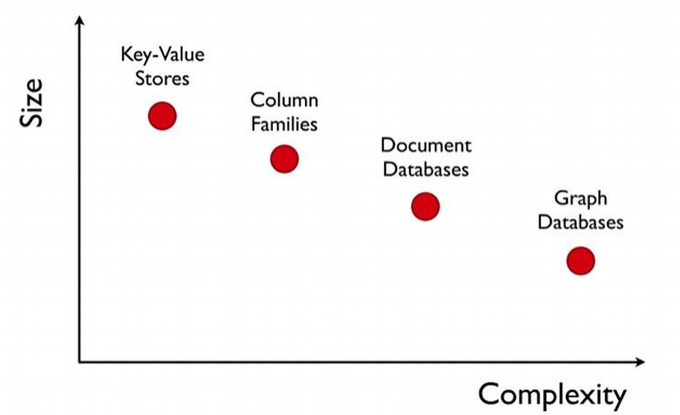
\includegraphics[scale=0.4]{IMAGE1.jpg}
\end{center}



\subsubsection{Document Based\cite{MongoDB}}
MongoDB è -come già affermato- un sistema di gestione basato sui documenti (document based management system), in cui i dati vengono storati in formato BSON (Binary JSON) e l'accesso ai dati stessi è possibile grazie all'esistenza di indici. Volendo fare un confronto con i database di tipo SQL, Mongo DB non prevedere la funzione join. Le principali differenze sono le seguenti:
\begin{center}
	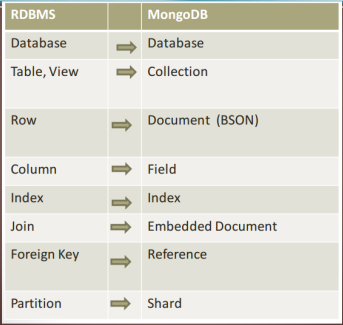
\includegraphics[scale=0.6]{IMAGE2.jpg}
\end{center}
Nel caso in cui si verifichi un massiccio caricamento di dati, si potrebbe decidere di apportare alcune modifiche al processo per fissarlo:
\begin{itemize}[noitemsep]
	 
	\item
	Disabilitare il riconoscimento dei dati, che è un segnale trasmesso tra processi di comunicazione, computer o dispositivi, per indicare il riconoscimento o la ricezione del messaggio, come parte di un protocollo di comunicazione
	\item
	Disabilitare la scrittura su un file di tipo log
\end{itemize}
Bisogna stare molto attenti nel fare ciò, perché ogni ogni perdita non sarà registrata e di conseguenza sarà persa per sempre.
\newline
Per grandi dataset risulta molto utile l'utilizzo di alcune strutture aggiuntive chiamate indici: simili agli indici dei libri, rappresentano un modo più veloce per recuperare informazioni.
Potrebbe essere richiesto più tempo durante la fase di inserimento degli stessi indici, ma questi renderanno l'esecuzione delle query molto più rapida. 
Un indice primario (basic one) è sempre quello definito per l'id. 

Ma come funziona esattamente?
Fondamentalmente, senza un indice, Mongo si comporterebbe come un semplice scansionatore di tabelle (esattamente come fa SQL). Dovrebbe di conseguenza cercare per tutto il ``libro'' al fine di trovare il risultato della query. L'analogia con il libro si esplicita al meglio nel seguente meccanismo: se non avessimo l'indice nei nostri libri, saremmo costretti a leggere il libro interamente fino a che non troviamo il paragrafo o il capitolo da cui siamo intenzionati a partire nella lettura. 
L'indicizzazione evita proprio questo problema (che risulta ancora più complicato se il database è ampio), fornendo una lista ordinata che indica il contenuto.
Dal momento che l'indicizzazione rallenta molto le modifiche, sarebbe necessario scegliere solamente una coppia di indici per ogni collection; la parte difficile è decidere quali. MongoDB dà, di default, un limite di 64 indici!

L'aggregazione utilizza pipeline e opzioni.
La pipeline di aggregazione avvia l'elaborazione dei documenti della raccolta (collection) e passa il risultato alla pipeline successiva per ottenere risultati, ad esempio: \ $ match e \ $ group.
Possiamo utilizzare lo stesso operatore in diverse pipeline.

Per molte ragioni (principalmente commerciali), Mongo offre anche un'interfaccia SQL; abbiamo bisogno del connettore BI (Business Intelligence): genera lo schema relazionale e usa tale schema per accedere ai dati.

\subsubsection{GraphDB\cite{Neo4J}}

Un grafo è una collezione di nodi e archi, i quali rappresentano le relazioni degli stessi nodi. 
Ha un sacco di applicazioni, come: social media, raccomandazioni, geo, reti logistiche, grafici per le transazioni finanziarie (per il rilevamento delle frodi), master data management, bioinformatica, autorizzazione e controllo degli accessi.
\newline
Il modello a grafo di proprietà con etichette (labeled-property graph model) ha le seguenti caratteristiche:

\begin{itemize}[noitemsep]
	 
	\item
	Contiene \textbf{nodi} e \textbf{relazioni};
	\item
	I nodi contiene \textbf{proprietà} (chiave : coppie di valori);
	\item
	I nodi possono essere etichettati con una o più \textbf{etichette};
	\item
	Le relazioni sono nominali e direzionali, con un nodo d'inizio e uno di fine;
	\item
	Come i nodi, anche le relazioni possono avere delle proprietà.
	\item
	%magari migliorare questa parte (Sicuramente fa pena nella lista)
	Le relazioni possono essere \textbf{fine-grained} or \textbf{generic}: \\Consideriamo il caso della relazione $Address$, si può fare distinzione tra:
	\begin{itemize}
		
		 \item le relazioni fine-grained come \texttt{HOME$\_$ADDRESS} o \texttt{WORK$\_$ADDRESS} o \texttt{DELIVERY$\_$ADDRESS} 
		 \item oppure potremmo scegliere solamente \texttt{ADDRESS} e specificare di quale tipo di indirizzo si tratta \texttt{ADDRESS\{type:`home'\}}. Questo metodo prende il nome di generic relationship. 
	\end{itemize}		 
	In genere si preferisce il generic, specialmente per quei casi in cui bisogna trovare tutti gli indirizzi di un cliente: tutto quello che basta fare è trovare la relazione \texttt{ADDRESS}, mentre nel caso del fine-grained sarebbe necessario trovare uno a uno tutti i tipi di indirizzi (immaginate di avere 100 tipi di indirizzo!). Con l'altro metodo (generic) per trovare il \texttt{DELIVERY$\_$ADDRESS} tutto ciò che bisogna fare è identificare \texttt{ADDRESS\{type:`delivery'\}}. 

\end{itemize}
Un database a grafo (Graph Database, GD) può usare sia un motore di archiviazione nativo o non-nativo (native or non-native storage) che un motore di elaborazione (processing engine).
\newline
L'archiviazione a grafo di tipo nativo è ottimizzata per la gestione a grafo nativa, mentre l'archiviazione a grafo di tipo non nativo tratta i dati in un modello non basato su grafico pur continuando a supportare un linguaggio di query grafico. Esempi sono: Relational, Object oriented DB, Wide Column. 
In un modello relazionale, per esempio, in una join bomb si può utilizzare un grafo per connettere due tabelle. 
Il problema con i database relazionali e la maggior parte dei database NoSQL è la mancanza di relazioni.
Inoltre in SQL le joining tables aggiungono un livello di complessità in più, e specialmente nel caso di tabelle scarse con colonne nulle l'operazione richiede un controllo speciale nel codice.
Nel caso di un mercato, solo per vedere cosa ha comprato un cliente, dobbiamo fare un sacco di joins costose sul cliente che ha comprato uno specifico prodotto con altri prodotti per il sistema di raccomandazione. 
For the NoSQL DBs, whether key-value, document or column-oriented, we might use the aggregation technique to see the relationship, but the relationship between aggregates aren't citizen in the data model. Indeed the aggregation is a costly operation since it doesn't exploit index free adjacency (the data is physically near) and since they stay inside of aggregates with structure in form of nested maps and even after the aggregation there is no back link to point backward and run
other interesting queries. 

In a native graph storage the attributes and nodes and the referenced nodes are stored together, to optimize the graph processing engine. 
Performing a query the graph-model, the response time does not strictly depend on the total number of nodes (it remains nearly constant) because the query is processed locally to the portion of the graph which is connected to the base node, while the other SQL and NoSQL models will suffer in performance speed with the increase of data. 
Moreover we can add more data/nodes and relationship without disturbing the already existing model.
\newline
The processing engine uses index-free adjacency, meaning that connected nodes physically points to each other in the DB, this makes sure that the retrieval is faster but it comes at a cost: the efficiency of queries that do not use graph traversal, for example the writing time etc.
\newline
It's important to note that it's neither good nor bad to use native or non-native engine, simply one needs to make a choice based on his/her needs. % for example my DB is based on a non-graph backend (like MySQL) so it would be useful to use a non native graph storage. 
\newline
Neo4j implements a declarative graph query language Cypher. Cypher allows graphs to be queried using simple syntax somewhat comparable to SQL or SPARQL, but particularly optimized for graph traversals.\\
The properties of the cypher language are:

\begin{enumerate}[noitemsep]
	 
	\item
	Pattern-matching query language
	\item
	Humane language, easy to learn, read and understand
	\item
	Expressive yet compact
	\item
	Declarative : Say what you want, not how
	\item
	Borrows from well known query languages especially SQL, yet clearly it's different enough to see that it deals with graphs and not SQL	DBs.
	\item
	Aggregation, Ordering, Limit
	\item
	Update the Graph
\end{enumerate}
\paragraph{A real example is the following}:\\ 
We want to manage a server farm, we define a relational model for managing it. 
We know that a user access to application which runs on a VM and each application uses a DB and a secondary DB. 
Each of the VM is hosted on a server placed in a rack structure managed by a load balancer.
\newline
The initial stage of modeling is similar in any kind of DB, we seek to understand and agree on the entities in the domain and how to interrelate, usually done on whiteboard with a diagram which is a graph.
Next stage we seek a E-R (Entity-Relationship) diagram, which is another graph. 
After having a suitable logical model we map it into tables and relations. 
We keep our data in a relational DB, with it's rigid schema.
But keeping the data normalized slows down the query time so we need to denormalize it, because the user's data model must suit the database engine not the user. 
By denormalizing we involve duplicate data to gain query performance: denormalization is not a trivial task and we accept that there may be substantial data redundancy. 
The problems do not stop here, because once the DB is created, if we need to modify it -this is typically going to happen in order to match the changes in the production environment- we will need to do the whole work again!
\newline
In these cases, It is better to directly use the graph DBs: it will avoid the data redundancy and it can adapt really fast in case of a change in the DB itself.
\newline
Another graph traversal language is Gremlin, part of the Apache TinkerPop framework. In this domain specific language (DSL) expressions specify a concatenation of traversal steps, so you basically explain to gremlin step by step what to do.

\subsubsection{Key-Value Model}

It's the most simple and flexible model of the NoSQL family, where every key is assigned to a value. It is possible to assign a type to a value.
The values are not query-able, such as a BLOB, where a BLOB(Binary Large OBject) is a collection of binary data stored as a single entity in a DB, for example images, videos etc.:
\begin{center}
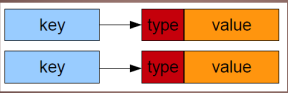
\includegraphics[scale=0.5]{IMAGE3.jpg}
\end{center}
An example is the amazon's cart system which uses DynamoDB, a key-value system.

~\\
The basic operation in a key-valued models are:

\begin{itemize}[noitemsep]
	\item
	Insert a new key-value pair
	\item
	Delete a new key-value pair
	\item
	Update a new key-value pair
	\item
	Find a value given the key
\end{itemize}
There is no schema and the values of the data is opaque. The values can be accessed only through the key, and stored values can be anything : numbers, string, JSON, XML, images, binaries etc.
An example of key-value model is Riak and has the following terminology:
%Quanto è figo minipage, l'ho scoperto dopo aver cercato come unire una tabella con un immagine xD!
\begin{center}
	\begin{minipage}[b]{0.4\textwidth}
	\begin{tabular}{|l|l|}
		\hline
		\textbf{Relational} & \textbf{Riak}\\ \hline
		database instance & Riak cluster\\ \hline
		table & bucket \\ \hline
		row & key-value\\ \hline
		rowid & key\\ \hline
	\end{tabular}
	\end{minipage}
	\begin{minipage}{.5\textwidth}\centering
	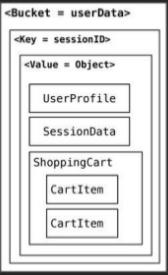
\includegraphics[scale=0.6]{IMAGE4.jpg}
	\end{minipage}

\end{center}
%Things not to remeber putting just for completation
Some other examples are: Redis, Memcached, Riak, Hazelcast, Encache.
\newline
Thanks to the Hash based index, the key-value systems can scale out in a very efficient way. 
The Hash is a mathematical function that assign to a given key it's value, usually we have $h(x) = value$, usually it returns a pointer to where the data is stored not exactly the data itself, for example $h(x) = (x\ modulo\ y)$ where $y$ is the max length of hash table. 
There might a problem with the conflicts but they can be managed. 
Hashing also enables items in the DB to be retrieved quickly. 
The hash table can be easily distributed in a network, it is managed in pile so we can have a key(saved in the pile) $x$ saved in a server and it's succ(x) stored in a different server, thus scaling out really fast. 
One reason to use hashing is so that we are able to
evenly distribute the data across a certain number of slots. If we want to hash any number into 10 buckets, we can use modulo 10; then key 27 would map to bucket 7, key 32 would map to bucket 2, key 25 to bucket 5, and so on.
%The key value terminology is the following:
\newline
In a DHT(Distributed Hash Table) it is pretty simple to insert a key-value \texttt{(k1,v1)}: basically take the key as input and route messages to the node holding that key and store the value there, and to retrieve the value of k1 the system simply finds the node with the key \texttt{k1} and return it's value \texttt{v1} from it.

\subsubsection{Wide Column and BigTable}
\paragraph{Intro to Columnar Storage:}%The idea that it might be better to store data in columnar format dates back to the 1970s, although commercial columnar databases did not appear until the mid-1990s. %maybe skippable
The essence of the columnar concept is that data for columns is grouped together on disk. In a columnar database, values for a specific column become co-located in the same disk blocks, while in the row-oriented model, all columns for each row are co-located. Indeed, one of the advantages to the columnar architecture is that queries seeking to aggregate the values of specific columns are optimized, because all of the values to be aggregated exist within the same disk blocks. The exact IO and CPU optimizations delivered by a column architecture vary depending on workload,indexing, and schema design. In general, queries that work across multiple rows are significantly accelerated in a columnar database.\\

These two models are an evolution, in a certain way, of the key-value models. When we start giving a structure to the value it becomes more complicated so we use wide column(Big Table): The first model was introduced by Google(HBase) and later on by Facebook (Cassandra), even though some consider Cassandra still  as a key-value model and not a wide column.

BigTable is a multidimensional map, which can be accessed by row key, column key and a timestamp. It is sorted, persistent and sparse.
We will consider the \textbf{HBase BigTable} Model.
The data is organized in tables, each table(the tables are multi-versioned) is composed by the column-families that include columns, the cells within a column family are sorted physically and are usually very sparse with most of the cell having \texttt{NULL} value so we can have different rows with different sets of columns. 
BigTable is characterized by the row key, column key, timestamp, the row has the keys, column contains the data and contents. 
The column is divided in families. The timestamp support the multi-version of modification to check how the data changed over time and still be able to access the latest one without any confusion. We can represent it as follows:

\begin{center}
	\begin{tabular}{|c|c|c|}
		\hline
		\textbf{row key} & \textbf{column family 1} & \textbf{column family 2} \\
		\hline
		&
		\begin{tabular}{c|c}
			\textbf{column 1} & \textbf{column 2}
		\end{tabular}
		&
		\begin{tabular}{p{1.8cm}|p{1.8cm}|p{1.8cm}}
			\textbf{column 1} & \textbf{column 2} & \textbf{column 3}
		\end{tabular}
		\\
		\hline
		&
		\begin{tabular}{c|c}
		\textit{cell(data)} & \textit{cell(data)}
		\end{tabular}
		& 
		\begin{tabular}{p{1.8cm}|p{1.8cm}|p{1.8cm}}
		\textit{cell(data)}&\textit{cell(data)} &\textit{cell(data)}
		\end{tabular}\\
		\hline
		&
		\begin{tabular}{c|c}
			\textit{cell(data)} & \textit{cell(data)}
		\end{tabular}
		& 
		\begin{tabular}{p{1.8cm}|p{1.8cm}|p{1.8cm}}
			\textit{cell(data)}&\textit{cell(data)} &\textit{cell(data)}
		\end{tabular}\\
		\hline
	\end{tabular}\\
	~\\
	Each row can have different timestamp, so we can have more versions of this table.
\end{center}
The data within the cells (also the key) has no type since it is saved in bytes. The columns are dynamic. So to get a data given a key we need to transform our data in Bytes with a comand .toBytes("Key"), we can also use python to modify the columns via APIs. This model can be useful for *-To-Many mappings.
The row key is an array of bytes and serves as a primary key for the table.
Each Column Family has a name and contains one or more related columns, the columns can belong to one column family only and is included inside the row with familyName:columnName followed the value, for example we have: \\ 
%cavolo che sbatti i quote i LaTeX, se trovate un modo carino ditemelo 
%take a look here! https://mirror.hmc.edu/ctan/macros/latex/contrib/csquotes/csquotes.pdf
row key $|$ info:\{`height':`170cm', `state':`NY'\}  roles:\{`ASF':`Director', `Hadoop':`Founder'\}$|$\\
The version number of each row is unique within the row key, by default it uses the system's timestamp but they can be user supplied.
\newline
Best time to use HBase is when one need to scale out, need random write and/or read, when we need to do thousand of operations per second on multiple TB of Data, when we need to know all the modification done on
the data, when we need a well known and simple access. One can combine a GraphDB with HBase, one example is JanusGraph.
HBase does not support joins, but this can be done in application layer using Scan() and Get() operations of HBase.
\newline
\newline
\textbf{Cassandra\cite{Facebook}}: It started as a support for the Facebook inbox search, it was open sourced in 2008 by Facebook and then it became a top-level project under Apache in 2010. The data model is the same as HBase, the only difference is the way it is stored (storage model) and the program algorithms. We can say it is a restricted BigTable, we can have only one column family. It uses a C* language very similar to SQL language.
\newline
Cassandra is a column oriented NoSQL system. 
The KeySpace is the outermost container, it's basic attributes are the Replication Factor (how many copies of the data we need), Replication Strategy and the Column Families.
The Column Families, can be seen as a collection of rows or better a collection of key-value pairs as rows. 
A row is a collection of columns labeled with a name, the value of a row is itself a sequence of key-value pairs where the keys are the column's name and we need at least one column in a row. The columns have the key(name), the value and the timestamp. So a table is a list of "nested key-value pairs": (ROW x COLUMN key x COLUMN value) and this is inside a column family.
The Key Space is only a logical grouping of columns families.

\begin{center}
	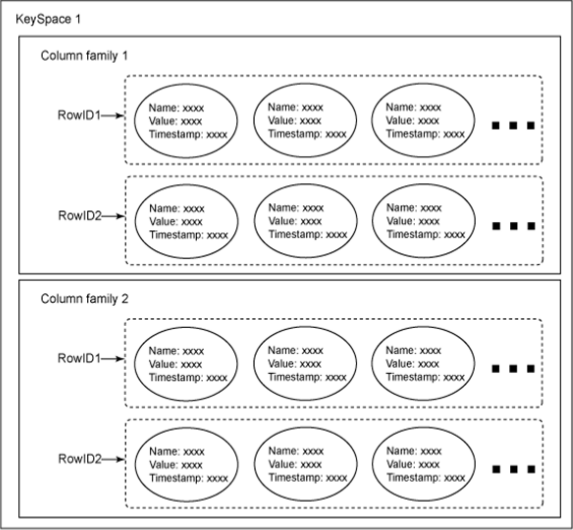
\includegraphics[scale=0.5]{IMAGE5.png}\\
	An example of Cassandra data model.
\end{center}
While with RDBMS, we can have that JOIN of normalized tables can return almost anything, with C* the data model is designed for specific queries and the schema is adjusted as new queries are introduced. In C* there are no JOINS, relationship or foreign keys and the data required by multiple tables are denormalized across those tables.
\newline
The Comparison between Apache Cassandra, Google Big Table and Amazon DynamoDB is:
\begin{center}
	\begin{tabular}{|p{3.6cm}|p{3.6cm}|p{3.3cm}|p{4cm}|}
		\hline
		&\textbf{Apache Cassandra} & \textbf{Google Big Table} & \textbf{Amazon DynamoDB}\\
		\hline
		\textit{Storage Type} & Column & Column & Key-Value\\
		\hline
		\textit{Best Use} & Write often\newline read less & Designed for\newline large scalability & Large database solution\\
		\hline
		\textit{Concurrency Control} & MVCC & Locks & ACID\\
		\hline
		\textit{Characteristics} & High Availability\newline Partition\newline Tolerance\newline Persistence & Consistency \newline High Availability\newline Partition\newline Tolerance \newline Persistence & Consistency \newline High Availability\\
		\hline
	\end{tabular}
\end{center}

\section{Data Distribution}
\subsection{Fragmentation and Replication}
Un sistema di DB centralizzato è un sistema in cui il database è localizzato, memorizzato e mantenuto in un'unica posizione. Se il processore fallisce, allora tutto il sistema fallisce.
Se abbiamo bisogno di avere dati periodicamente in luoghi differenti allora possiamo distribuirli o replicarli. La distribuzione quindi consiste nel dividere i dati e memorizzarli in posti diversi, provvedendo così ad avere possibilità di eseguire operazioni in parallelo. D'altra parte possiamo anche replicarli (interamente o solo una parte) in diversi luoghi, migliorando cosi la loro disponibilità (availability).
\newline
In un Database Distribuito Omogeneo tutti i siti hanno identico software e concordano tutti a collaborare per l'elaborazione delle richieste dell'utente. Si arrendono alla loro autonomia per cambiare lo schema che appare all'utente come un singolo sistema.
\newline
In un Database Distribuito Eterogeneo diversi siti possono usare differenti schemi e software, creando maggior problemi per query e transazioni. I siti possono non essere a conoscenza l'uno dell'altro e quindi potrebbero fornire solo strutture limitate per la cooperazione nell'elaborazione delle transazioni.
\newline
Le sfide per la progettazione di un Database Distribuito sono decidere cosa va, che dipende dal pattern di accesso ai dati, e dal problema di dove allocare i frammenti ai nodi.
Con la replicazione il sistema mantiene multiple copie dei dati, memorizzate in diversi siti, per un veloce recupero e tolleranza degli errori con la frammentazione dei dati divisi in frammenti archiviati in siti diversi. Possiamo combinare entrambi, in modo che i dati siano partizionati in diversi frammenti, e che il sistema mantenga diverse repliche degli stessi.
\newline
Dividendo/frammentando il nostro database in n database, sorge il fenomeno "bottle-neck", dove la macchina più lenta detta la peggior performance per una query.
\newline
I vantaggi di una replicazione sono:
\begin{itemize}[noitemsep]
	\item
	Availability: l'errore di un sito non determina l'indisponibilità dei dati, in quanto la sua replica esiste altrove.
	\item
	Parallelism: le query possono essere processate da diversi nodi parallelamente, rendendo tutto più veloce.
	\item
	Reduced data transfer: poiché possono esistere repliche dei dati nel nodo stesso.
\end{itemize}

Mentre gli svantaggi sono:

\begin{itemize}[noitemsep]
	 
	\item
	Aumentati i costi per gli update: in quanto ogni replica deve essere aggiornata.
	\item
	increased complexity of concurrency control e.g. due persone prendono lo stesso ticket nello stesso istante. Potremmo avere che repliche distinte possono portare a dati incoerenti a meno di qualche meccanismo di concurrency speciale venga implementato. Una soluzione potrebbe essere quella di scegliere una copia come copia primaria e applicare operazione di controllo della conucrrency solo sulla copia primaria.
\end{itemize}
Come già accennato, possiamo combinare la replica dei dati con la frammentazione dei dati. In particolare la frammentazione dei dati consiste in una divisone di relazioni r in frammenti che contengono sufficienti informazioni per ricostruire la relazione r.
Ora per semplicità, immaginiamo che sia un database relazionale. 
La frammentazione può essere orizzontale o verticale, l'importante che contenga informazioni sufficienti per ricostruire la "relazione" originale . In quella orizzontale ogni tupla deve essere assegnata a uno o più frammenti mentre nella frammentazione verticale, lo schema è splittato in due diversi schemi più piccoli, dove entrambi devono contenere una chiave comune per assicurare un join senza perdite, per esempio utilizzando una tupla-ID come attributo.\newline
I vantaggi sono:
\begin{itemize}[noitemsep]
	\item Orizzontale:
	\begin{itemize}[noitemsep]
		\item Permette processi paralleli sui frammenti.
		\item Permette lo split dei dati in modo che le tuple siano poi allocate nei posti in cui avviene l'accesso più frequentemente.
	\end{itemize}
	\item Verticale
	\begin{itemize}[noitemsep]
		\item Permette alle tuple di essere splittate in modo che ogni parte delle tuple sia archiviata nel luogo in cui avviene più spesso l'accesso.
		\item tuple-id permette un efficiente join di frammenti verticali.
		\item Permette processi paralleli su una relazione.
	\end{itemize}
\end{itemize}
Le due frammentazioni possono essere mixate insieme, e inoltre i frammenti possono essere successivamente frammentati fino ad una profondità arbitraria. 
Data Transparency è veramente importante perché indica il grado per cui un utente non è consapevole di come i dati sono stati archiviati in un sistema distribuito. Dobbiamo considerare i problemi sulla transparency in relazione a: frammentazione, replicazione e location dei nostri dati.
\newline
Considerando la differenza tra un sistema centralizzato e uno distribuito, dal punto di vista dei costi, abbiamo che:
\begin{itemize}[noitemsep]
\item Per un sistema centralizzato, il criterio principale per misurare il costo di una particolare strategia è il numero di accesso ai dischi.
\item In un sistema distribuito dobbiamo invece considerare il costo per la trasmissione dei dai sulla rete  e anche il potenziale guadagno in performance che si ottiene con l'ausilio dei diversi siti che entrano nel processo svolgendo query parallele.
\end{itemize}
Ricapitolando abbiamo che i vantaggi dei DDBMSs sono: riflette la struttura organizzativa migliorando determinate caratteristiche tra cui l'abilità di condivisione, autonomia locale, la disponibilità, l'affidabilità e la performance, riducendo il costo dell'hardware grazie anche ad una crescita modulare .
Gli svantaggi sono: architettura e progettazione più complessa e costosa; la sicurezza e l'integrità sono più difficilmente controllabili; c'è una mancanza di standard ed esperienza nel suo utilizzo.
\newline
Ci sono 3 tipi di architetture nei DDBMS:
\begin{itemize}
\item Shared Everything: dominata dal mercato delle architetture fino al 2000(circa), abbiamo un grande e costoso database, che condivide ogni cosa, per cui molto lento; è il sistema centralizzato.

\item Share Disk: abbiamo i dati salvati su diversi dischi connessi tra loro. I dischi sono tutti connessi insieme e comunicano con tutte le CPUs.

\item Share Nothing: ogni cosa è separata, ogni disco ha la propria CPU e non comunica con le altre CPU o dischi; solo alla fine i processori vengono connessi insieme per combinare i risultati da ognuno di essi; Il modello è adottato dai modelli NoSQL; è molto facile lo scale out. 
\end{itemize}

\begin{center}
	\begin{tabular}{|c|c|}
		\hline
		\textbf{Shared Disk} & \textbf{Shared Nothing}\\
		\hline
		Quick adaptability to changing workloads & Can exploit simpler, cheaper hardware\\
		\hline
		High availability & Almost unlimited scalability\\
		\hline
		Performs best in a heavy read environment & Works well in high-volume, read/write environment\\
		\hline
		Data need not to be partitioned & Data is partitioned across the cluster\\
		\hline
	\end{tabular}
\end{center}
Cosa scegliere tra Scalability o Availability? Dipende da quanto vogliamo spendere: più availability significa più denaro. Per esempio una disponibilità del 100\% significa nessun down del sistema; diminuendo la disponibilità e quindi aumentando i down, potremmo avere disponibilità 99\% con down compresi tra le 9 - 88 ore.
\newline
\textbf{Replication}:
\newline
Un log è un file sequenziale che è storato in una memoria stabile (che non dà mai errore; esso archivia tutte le attività realizzate dalle
transazioni in ordine cronologico. Ci sono due tipi di record: transaction logs(operations) e system event (Checkpoint and Dump).
Possiamo definire un checkpoint, quel momento in cui noi memorizziamo un set di transazioni in un dato tempo, mentre un dump è una copia piena dello stato di un DB in una memoria stabile; la sua esecuzione è offline, e genera un backup. Solo dopo che il backup è completo, che il dump recod viene scritto nel log.
\newline
Le strutture di replica sono:
\begin{itemize}[noitemsep]
	\item One2Many: una sorgente e alcuni target.
	\item Many2One: alcune sorgenti e un solo target.
	\item Peer2Peer: i dati sono replicati attraverso molteplici nodi che comunicano l'uno con l'altro.
	\item Bi-directional: concettualmente un Peer2Peer con solo due Peers.
	\item Multi-Tier Staging: la replicazione è divisa in più stages.
\end{itemize}

Per creare una replica possiamo:
\begin{itemize}[noitemsep] %qua mi sfugge qualcosa (CONTROLLARE)
	\item Prendere i dati dal master, sia il backup o i dati stessi (se vogliamo stoppare l'attività del server) e muoverli (potrebbe essere utile se i dati non sono accessibili dall'esterno).
	\item use log file : per mantenere la replica uguale alla sorgente durante il trasferimento (quasi in tempo reale) si usa il Log per eseguire gli stessi comandi eseguiti sulla sorgente.
\end{itemize}


%If you use Volume in project be attentive to the scalability!!!!!
\subsection{MongoDB's Approach: Sharding\cite{ScalingMongoDB}}

MongoDB usa lo Sharding per splittare una grande collezione in diversi server (chiamati cluster); ogni documento ha una chiave in mongodb, noi definiamo una chiave che definisce il range dei dati (chunk range).
Gli spazi nella chiave sono come punti su una linea, mentre il range è il segmento di quella linea.
Esempio: la chiave è il cognome, quindi decidiamo che tutti i cognomi che iniziano tra A e K vengano salvati in una partizione mentre gli altri in una seconda.
MongoDB non fa lo shard automaticamente una volta che abbiamo deciso di distribuire i dati. 
Di default la massima dimensione del chunk è di 64Mb; se tende ad aumentare la dimensione del chunk, MongoDB automaticamente lo splitterà in due più piccoli chunk, e se gli shard diventano sbilanciati, allora alcuni chunk migreranno ad altri shard cercando di correggere questo sbilanciamento. 
L'obiettivo del bilanciamento non è solo quello di mantenere ugualmente distribuiti i dati, ma è anche quello di minimizzare l'ammontare dei dati trasferiti. 
Il bilanciamento è piuttosto pigro, quindi non si attiva fino a quando i dati non sono molto squilibrati; lo fa per cercare di
evitare lo spostamento di dati avanti e indietro, nel caso in cui dovesse bilanciare ogni minima differenza (si sprecherebbero troppe risorse)
\newline
Quando crei uno shard, MongoDB crea un singolo chunk con range $(-\infty, +\infty)$ dove con $-(+)\infty$ intendiamo il più piccolo/massimo valore che MongoDB può rappresentare. 
Da qui, se la dimensione del chunk è più grande di quella scelta, allora verrà splittata; ogni chunk range dovrà essere distinto e non sovrapposto, e inoltre la loro unione dovrà coprire il range iniziale.
\newline
Lo shard è in pratica un server, quindi bisogna usare mongos (s=server) per fare una query. Mongos è il punto di interazione tra l'utente e il cluster, che ti permette di trattare un cluster come un singolo server.
Le query vengono instradate verso l'apposito shard grazie a mongos. Per le query senza target (es: with sorting) una richiesta è mandata a tutte le shard, e le query sono elaborate localmente; dopo che il risultato è ritornato, mongos mergia il risultato sorted e manda al client il risultato finale.
Mongos attualmente non archivia alcun dato; la configurazione di un cluster è mantenuta in uno speciale mongods, chiamato config server, che tiene le informazioni circa gli accessi di chiunque a quel cluster.
\newline
Il cluster consiste in tre tipi di processi:
\begin{itemize}[noitemsep]
	\item The shards: un nodo del cluster, può essere sia un singolo mongod che un set replica. MongoDB in automatico replica i dati in una shard dove avremo il chunk primario (con i dati storati che volevamo), e un chunk secondario dove vengono reolicati i dati come backup (è solo in lettura, non si possono fare query).
	\item Mongos processes: serve per guidare le richieste verso la posizione dei dati, e agisce come bilanciamento dei chunks. Non contiene dati locali. Possono esserci uno o più processi. Dopo che il bilanciamento è finito, il processo aggiorna anche il Config Servers con la nuova posizione e intanto il mongos che sta bilanciando i chunks, tira fuori un "balancer-lock", in modo che nessun altro mongos incomincerà il bilanciamento, che era già ultimato. Il lock è rilasciato solo dopo che il chunk è stato copiato, e il vecchio chunk cancellato dallo shard iniziale.
	\item Config servers: per mantenere traccia dello stato dei cluster. Archivia il chunk range e la posizione dei cluster. Si possono avere solo 1 o 3.
\end{itemize}

\begin{center}
	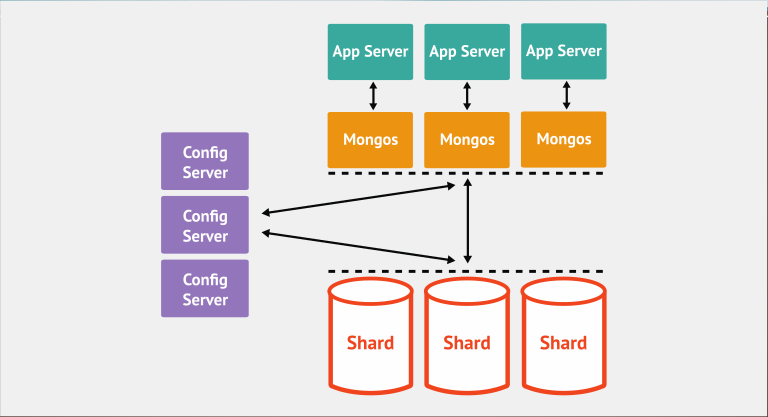
\includegraphics[scale=0.40]{IMAGE6.png}
\end{center}


Let's see the steps for the configuration:

\begin{enumerate}[noitemsep]
	\item Start a config server, it start by default at port 27019:

	mongod --configsvr
	\item Start the mongos Router, we need to initialize it like this even if the cluster is already running:
	
	For 1 configuration server: 
	mongos --configdb $<$hostname$>$:27019
	
	For 3 configuration servers:
	mongos --configdb $<$host1$>$:$<$port1$>$,$<$host2$>$:$<$port2$>$,$<$host3$>$:$<$port3$>$
	
	We can have different mongos on same pc on different ports.
	\item Start the shard database, it starts a mongod with the default shard port 27018
	
	mongod --shardsvr
	
	The shard is not yes connected to the rest of the cluster and it may have been already running in production.
	\item Add the Shard:
	
	On mongos: 
	sh.addShard('$<$host$>$:27018')
	
	To add a replica set: 
	sh.addShard('$<$rsname$>$/$<$seedlist$>$')
	\item Verify that the shard was added:
	
	db.runCommand(\{ listshards:1 \}) \newline
	Obtaining as result: \newline
	\{\newline
	"shards": \newline
	[\{ "\_id":"shard0000", "host":"$<$hostname$>$:27018"\}], \newline
	"ok" : 1 \newline
	\}
\end{enumerate} 
To enable sharding on a database simply use the command: sh.enableSharding("$<$dbname$>$") 
\newline To start a collection with the given key:
sh.shardCollection("$<$dbname$>.$people",\{"country" : 1\})
\newline
Le proprietà di una Shard Key sono:
\begin{itemize}[noitemsep]
	\item Shard key è immutabile
	\item Shard key values sono immutabili
	\item Shard key deve essere indicizzato
	\item Shard key sono limitati a dimensioni massime di 512 bytes
	\item Shard key sono usate per guidare le query: scegliendo un campo comunemente usato in query
	\item Solo la shard key può essere unica tra le shards (the `\_id' field is only unique within the individual shard)
\end{itemize}

\subsection{HBase}
We can consider HBase tables as potentially massive tabular datasets that are implemented on disk by a variable number of HDFS files called Hfiles.
All rows in an HBase table are identified by a unique row key. A table of nontrivial size will be split into
multiple horizontal partitions called \textbf{regions}. Each region consists of a contiguous, sorted range of key values (reminding of the MongoDB range-based sharding scheme).

Read or write access to a region is controlled by a \textbf{RegionServer}. There will usually be more than one region in each RegionServer. As regions grow, they split into multiple regions based on configurable policies (may also be split manually).

Each HBase installation will include a Hadoop \textbf{Zookeeper service} that is implemented across multiple nodes.
Hbase may share this Zookeeper ensemble with the rest of the Hadoop cluster or use a dedicated service. %When an HBase client wishes to read or write to a specific key value, it will ask Zookeeper for the address of the RegionServer that controls the HBase catalog. The client will then establish a connection with that RegionServer and request to read or write the key value concerned. %extras?

The HBase \textbf{master server} performs a variety of housekeeping tasks. In particular, it controls the
balancing of regions among RegionServers. If a RegionServer is added or removed, the master will organize for its regions to be relocated to other RegionServers. An HBase client consults Zookeeper to
determine the location of the HBase catalog tables, which can be then be interrogated to determine the
location of the appropriate RegionServer. The client will then request to read or modify a key value from
the appropriate RegionServer. The RegionServer reads or writes to the appropriate disk files, which are
located on HDFS. %taken almost literally from the suggested course book "Next Generation DB"

Summing up, the four major components (nodes) of HBase are:
\begin{enumerate}[noitemsep]
	\item The HMaster (only one): It is the implementation of Master server in HBase architecture. It monitors and coordinates all slaves in the cluster. It must assign regions, detect failures and has admin privileges. 
	\item The HRegionServer (many of them): It manages the data regions and serves client requests for reads and writes (using a log), this request is assigned to a specific region, where actual column family resides. However the client can contact directly the HRegionServer without having a permission of HMaster. HMaster is required only for operations related to metadata and schema changes. The Region servers run on Data Nodes present in the Hadoop cluster.\newline
	The HRegions are the basic building elements of HBase cluster that consists of the distribution of tables, i.e., a subset of a table's rows, like horizontal range partitioning and it is done automatically.
	\item The HBase client
	\item Zookeeper: It is a centralized monitoring server which maintains configuration information and provides distributed synchronization between nodes.
	HBase lives and depends on ZooKeeper, by default HBase manages the ZooKeeper instance (start and stop). 
	HMaster and HRegionServers register themselves with ZooKeeper.
	If the client wants to communicate with regions, the servers client has to approach ZooKeeper first.
	During a failure of nodes ZooKeeper Quoram will trigger error messages, and it starts to repair the failed nodes.
\end{enumerate}
HBase's architecture is similar to MongoDB's and they share the same flaw: If the master is broken the client cannot obtain any data and we have an error (Single point of failure).

\subsection{Cassandra}
In Cassandra there are no specialized master nodes. Every node is equal and every node is capable of performing any of the activities required for cluster operation. \footnote{Nodes in Cassandra do, however, have short-term specialized responsibilities. For instance, when a client performs an operation, a node will be allocated as the coordinator for that operation. When a new member is added to the cluster, a node will be nominated as the seed node from which the new node will seek information. However, these short-term responsibilities can be performed by any node in the cluster.}
It uses a peer-to-peer distributed system. 
The Data is partitioned among all nodes in the cluster and a custom data replication to ensure fault tolerance and since all the nodes are all considered same we have Read/Write-anywhere design.
Cassandra is based on Google BigTable and Amazon Dynamo so it inherits their properties.
\newline
In Cassandra we can add or remove nodes with no downtime so we have a transparent elasticity and transparent scalability (performance grows linearly with the number of nodes) and due to it's P2P architecture we obtain also the High Availability. If a node were to fault we will have that we could obtain the data from the replicas in the other nodes.
The Nodes are logically structured in Ring Topology, the hashed value of key associated with data partition is used to assign it to a node in the ring. The hashing rounds off after a certain value to support the ring structure and the lightly loaded nodes moves position to alleviate the highly loaded nodes.
Cassandra uses ZooKeeper to find the replicas in other nodes, given a node we decide the N number of following nodes in which the replica will be saved.
%%%


\begin{figure}
\centering
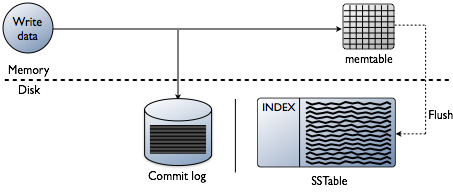
\includegraphics[width=100 mm]{cassandrawrite.png}
\caption{\label{cassandrawrite:fig} Data writing procedure in Cassandra.}
\end{figure}
As illustrated in Fig.~\ref{cassandrawrite:fig}, The data writing is separated in 3 stages : 
\begin{enumerate}
	\item The log file writing, which is essential: even if the data writing fails it doesn't matter because we have the log file.
	\item Once written in the commit log, data is written to the mem-table. Data written in the mem-table on each write request also writes in commit log separately. Mem-table is a temporary storage of data in the memory while commit log logs the transaction records for backup.
	\newline The first place where the read operations take place is mem-table and several may exist at once (1 current and other waiting to be flushed). 
	\item When mem-table is full, flush the data from the mem-table and store them disk in SSTables. The SSTables are immutable once written.
\end{enumerate}
The consistency can be based on majority: if a certain number,which we decide(it can also be one), of the nodes agree that a certain data was written or read it is assumed to be true; \newline
or it can be based on quorum which states the $50\%\text{(of the replication factor)}+1$ nodes agree that something is written it's assumed true.
\newline
The commands for writing for write consistency one(quorum): \newline
INSERT INTO table (column1, ...) VALUES (value1, ...) USING CONSISTENCY ONE (QUORUM)\newline
If a node is offline, an online node makes a note to carry out the write once the node comes back online.
For reading the data we have the following command:
SELECT * FROM table USING CONSISTENCY ONE
\newline
To delete the data is it easier to consider the data not available and mark it for deletion, it is called a tombstone(like how recycle bin works in OS), and actually delete on a major compaction or configurable timer.\newline
Compaction runs periodically to merge multiple SSTables reclaiming space, creating new index, merging the keys, combining columns and discarding the tombstones.

One of the advantages of a master node is that it can maintain a canonical version of cluster
configuration and state. In the absence of a master node keeping a canonical version of cluster configuration, Cassandra requires that all members of the cluster be kept up to date with the current state of cluster configuration and status. This is achieved by use of the \textbf{gossip protocol}. Every second each member of the cluster will transmit information about its state and the state of any other nodes it is aware of to up to three other nodes in the cluster. One nodes gossip about other nodes as well as about their own state.
This architecture eliminates any single point of failure within the cluster.\footnote{Although distributed databases with master nodes have strategies to allow for rapid failover, the crash of a master node usually creates a temporary reduction in availability, such as momentarily falling back to read-only mode.}

One of the main reasons of gossip is related to node availability. Usually the only way to detect node failure is a system of heartbeats between nodes. However (in a distributed system) the heartbeats may be lost because of network issues rather than actual node failure. Cassandra failure detection is more probabilistic: nodes in the cluster become increasingly "worried" about other nodes, and if it seems likely that a node is down the operations will be redirected.

Cassandra distribute data throughout the cluster by using \textbf{consistent hashing}. The rowkey (analogous to a primary key in an RDBMS) is hashed. Each node is allocated a range of hash values, and the node that has the specific range for a hashed key value takes responsibility for the initial placement of that data.
We usually visualize the cluster as a ring: the circumference of the ring represents all the possible hash values, and the location of the node on the ring represents its area of responsibility. 
When adding a new node, the system remaps all
the hash ranges (exploiting a peculiar mechanism of Virtual node to optimize this operation)\footnote{More infos in the suggested course text-book}.

%Sezione in italiano ricavata dagli appunti dell'anno scorso. (Grande)
%Per ora non si sa se questa parte sarà richiesta all'esame. Adesso sì
%Da integrare se disponete di appunti affidabil ricavati a lezione
\section{Big Data Architecture}
La prima definizione di "Big Data" viene data da Gartner nel 2012: "Big data is high volume, high velocity and/or high variety information assets". Ad oggi sappiamo però che per definire i "Big Data" potremmo usare più di 3 V, aggiungendo anche variability e veridicity. Analizzare "Big Data" su un singolo server "big" è un processo lento, costoso e difficile da realizzare. La soluzione è effettuare un’analisi distribuita su hardware poco costosi tramite un sistema di calcolo parallelo, i cui vantaggi sono già stati esposti nella sezione dedicata all'architettura distribuita. I problemi principali della distribuzione dei dati sono la sincronizzazione, i cosiddetti "punti morti" (deadlock), la larghezza della banda, la coordinazione tra i nodi e i casi di fallimento (failure) del sistema. Questo genere di architettura ha comunque molti vantaggi, tra cui: scala linearmente (scale out), l’attività di calcolo è rivolta ai dati e non viceversa (cambio di paradigma), gestisce i casi di fallimento (failure) e lavora con hardware con potenza di calcolo "normale".
\subsection{HDFS}
L’architettura HDFS (Hadoop Distributed File System) è un file system distribuito progettato per girare su hardware base (commodity hardware).
\begin{center}
	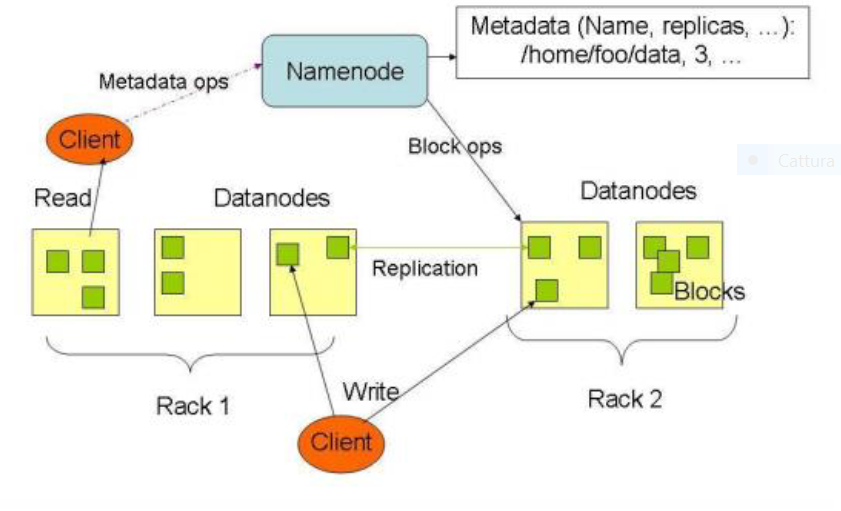
\includegraphics[scale=0.70]{IMAGE7.png}\\
	HDFS Architecture
\end{center}
Sebbene ci siano molte similitudini con altri sistemi di file system distribuiti, le differenze sono comunque significative. In particolare, HDFS è fortemente tollerante agli errori
ed è progettato per girare su macchine poco costose, inoltre fornisce un accesso ad alta velocità ai dati delle applicazioni ed è ideale per applicazioni con data set di grandi dimensioni. HDFS ha un’architettura master/slave. Un cluster HDFS consiste in un singolo NameNode e in un server master che gestisce il file system detto NameSpace e che regola gli accessi ai file da parte dei clients (secondo modello di accesso $Write-once-Read-many$). Inoltre, sono presenti un certo numero di DataNodes, generalmente uno per ogni nodo nel cluster, che gestiscono lo storage collegato ai nodi su cui vengono eseguiti. Internamente, un file è splittato in uno o più blocchi (tipicamente di 128 MB ciascuno) e questi sono memorizzati in un set di DataNodes. Il NameNode esegue le operazioni del file system NameSpace, ovvero apertura, chiusura e "rename" dei file e delle directories. Inoltre, determina la mappatura dei blocchi nei DataNodes, e reindirizza le richieste di operazioni di lettura e scrittura da parte del file system dei clients ai DataNodes. I DataNodes permettono anche la creazione, l’eliminzazione e la replica dei blocchi sotto istruzioni del NameNode. I Meta-Data (lista dei file, lista dei blocchi, lista dei DataNodes, attributi del file, …) sono tutti memorizzati nella memoria principale. Esiste inoltre un Transaction Log che registra la creazione, l’eliminazione e qualunque altra operazione avvenga su un file.
La strategia di piazzamento dei blocchi del file tra i DataNodes è la seguente:
\begin{itemize}[noitemsep]
\item Una replica sul nodo locale
\item Una seconda replica su un rack (collezione di nodi) remoto
\item Una terza replica sullo stesso rack remoto
\item Delle repliche piazzate in modo randomico
\end{itemize}
I client leggeranno il file dalla replica più vicina a loro (rack awareness). Esiste poi un sistema per verificare la correttezza dei dati. Può succedere infatti che un blocco inviato dal DataNode arrivi corrotto. Il client software HDFS implementa un controllo checksum dei file. Quando un utente crea un file, genera anche un checksum per ogni blocco del file e memorizza questi checksum in un file nascosto separato nello stesso NameSpace HDFS. Quando un client richiede l’accesso al file, verifica che i dati ricevuti da ogni DataNode combacino con il checksum associato. Se così non è, il client deciderà di reperire quel determinano blocco da un altro DataNode che possiede una replica di tale blocco di dati. Il NameNode verifica inoltre che i DataNodes, i quali inviano continuamente "segnali di vita", siano tutti funzionanti e gestisce gli eventuali malfunzionamenti. Tuttavia, il NameNode rappresenta un "single point of failure". Per questo motivo i Transaction Log sono memorizzati in più directrories: nel file system locale e in uno remoto.\newline
Formati di file supportati: Text, CSV, JSON, SequenceFile, binary key/value pair format, Avro*, Parquet*, ORC, optimized row columnar format.

\subsection{Map Reduce}
Map Reduce è un motore di computazione distribuito. Ogni programma è scritto in stile funzionale ed è eseguito in parallelo. "Mapred" risolve problemi legati alla gestione di processi di gestione/processing di BigData (ad esempio distributed pattern-based searching, distributed sorting) quali:
\begin{itemize}[noitemsep]
\item Come assegnare i 'lavori' ai singoli 'worker'
\item Cosa succede se ci sono più 'lavori' che 'worker'
\item Cosa succede se i 'worker' devono condividere risultati parziali
\item Come aggregare i risultati parziali
\item Come scoprire se tutti i 'worker' hanno finito il proprio task
\item Cosa succede se un 'worker' muore
\end{itemize}
\begin{center}
	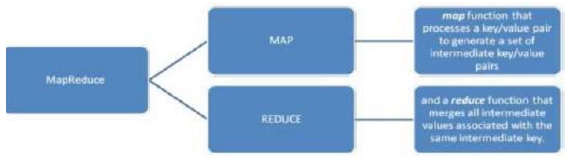
\includegraphics[scale=1]{IMAGE8.png}\\
	Map Reduce
\end{center}
La fase di Map esegue lo stesso codice su un grande ammontare di record, estrae le informazioni rilevanti, le ordina e le unisce. La fase di Reduce aggrega i risultati intermedi e genera l’output. Il programmatore dovrà esclusivamente definire le due funzioni di map (\texttt{map (k, v) -> [(k’, v’)]}) e di reduce (\texttt{reduce (k’, [v’]) -> [(k’, v’)]}). Tutte le altre attività le svolge  $MapRed$.
\subsection{Hadoop}
Hadoop è un framework che supporta applicazioni distribuite con elevato accesso ai dati, unisce il sistema MapReduce (parallel and distributed computation) e l’HDFS (hadoop storage and file system).
\begin{center}
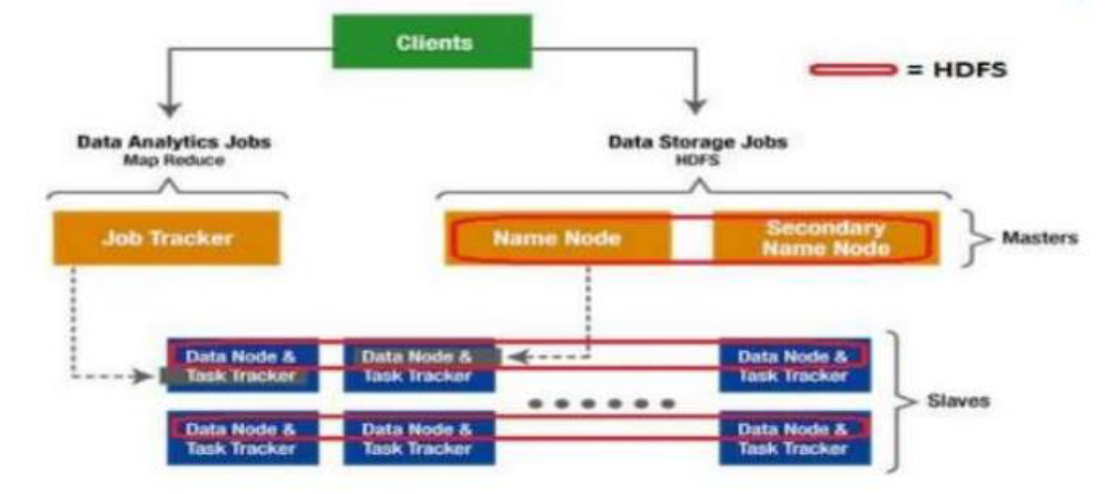
\includegraphics[scale=0.70]{IMAGE9.png}\\
Schema ecosistema Hadoop
\end{center}
Main features\footnote{From "Next Generation
Databases", Guy Harrison.} %maybe add to bibtex if doesn't exist yet?
\begin{itemize}

 \item It is an economical scalable storage model. As data volumes increase, so does the cost of storing that data online.
 Because Hadoop can run on commodity hardware that in turn utilizes commodity disks, the price point per terabyte is lower than that of almost any other technology.
\item Massive scaleable IO capability. Because Hadoop uses a large number of
commodity devices, the aggregate IO and network capacity is higher than that
provided by dedicated storage arrays in which smaller numbers of larger disks are provided by even smaller numbers of processors.\footnote{Furthermore, adding new servers to Hadoop adds storage, IO, CPU, and network capacity all at once, whereas adding disks to a storage array might simply exacerbate a network or CPU bottleneck within the array.}
\item Reliability: Data in Hadoop is stored redundantly in multiple servers and can be distributed across multiple computer racks. Failure of a server does not result in a loss of data; in fact, a Hadoop job will continue even if a server fails—the processing simply switches to another server.
\item A scalable processing model: MapReduce.
\item Schema on read: Data can be loaded into Hadoop without having to be converted
to a highly structured normalized format. This makes it easy for Hadoop to quickly ingest data from various forms. The imposition of structure can be delayed until the data is accessed; this is sometimes referred to as schema on read, as opposed to the schema on write mode of relational data warehouses.
\end{itemize}
\subsubsection{The Hadoop Ecosystem}
L'ecosistema di Hadoop include una famiglia di utiliy e applications sempre in espansione, costruita sopra o progettata per lavorare con il core di Hadoop (Yarn, HDFS).

Pig è uno scripting language che esegue l’analisi dei dati. Gli script in "pig latin" sono tradotti in lavori di MapRed. 

Hive è un’interfaccia simile a SQL per dati memorizzati in HDFS. I piani di esecuzione sono generati automaticamente da Hive. Hive rappresenta quindi un data warehousing basato su Hadoop. Questo applicativo è utilizzato per report giornalieri, misure di attività degli utenti, data e text mining, machine learning e per attività di business intelligence come pubblicità e individuazione degli spam.

Tuttavia, il sistema di MapRed ha dei limiti: è difficile da comprendere, i task non sono riutilizzabili, è incline agli errori e per analisi complesse richiede molti lavori di MapReduce. In Hadoop 1.0 dunque, ogni "jobtracker" deve gestire molti compiti: gestire le risorse computazionali, scandire i task dello stesso lavoro, monitorare la fase di esecuzione, gestire i possibili "failure" e molto altro ancora. La soluzione a questo problema è stata splittare la fase di gestione in gestione dei cluster e gestione dei singoli lavori. Questo sistema è stato messo in pratica da YARN (Yet Another Resource Negotiator) in cui è presente un ResourceManage globale e un ApplicationMaster per ogni applicazione.

Vengono rilasciati inoltre altri applicativi quali Accumulo, Hbase e Spark \footnote{If we think about Hadoop as a disk-oriented framework for running MapReduce-style programs, Spark represents a memory-oriented framework for running similar workloads}, Kafka (distributed streaming messaging system), Oozie (workflow scheduler that allows complex workflows to be constructed from lower level jobs).
In Cloudera sono presenti anche Impala, Mahout (machine-learning framework), Sqoop (utility per scambiare dati con relational databases, in import o export) e Flume (utility for loading file-based data (i.e. web server logs) into HDFS) 

\subsection{Data Lake}
Il termine "data lake" è stato coniato nel 2010 da James Dixon, il quale ha distinto due approcci di gestione dei dati: Hadoop e i data warehouses. Quest’ultimo (anche detto data mart) consiste nel memorizzare i dati in modo pulito e strutturato per una facile "consumazione" futura.

Un data lake invece è una struttura capace di contenere un enorme quantità di dati salvati in ogni formato, in maniera non costosa.
\`E una soluzione infrastrutturale in cui lo schema e i requisiti dei dati non sono definiti in partenza, ma vengono delineati al momento dell'interrogazione ($query\ time$): si tratta dello $schema\ on\ read$, caratteristico di un approccio "bottom up", caratterizzato dall'osservazione "sperimentale" come motore di un processo induttivo. 
Da questo "lago" ogni soggetto (autorizzato) può attingere, tipicamente passando per un processo di analisi e di campionamento accurato. 
Può avere lo scopo di catturare tutti i dati forniti in fase di "ingestion", e di passare solo quelli ritenuti rilevanti ad una Enterprise Data Warehouse (EDW): può essere quindi una fonte di dati per questa EDW. In questo modo si risparmia risorse relative all'EDW, e permette un'esplorazione iniziale dei dati disponibili, senza modellazione da parte dell'EDW team ($quick\ user \ access$).
Una delle caratteristiche salienti del Data Lake è inoltre la facile scalabilità. 
%sorry for the language swapping, but it's somehow easier this way
As reported in Fig.~\ref{data_lake_arch:fig}, components of a typical data lake architecture are\footnote{See also \url{http://www.oreilly.com/data/free/files/architecting-data-lakes.pdf}. Note a slightly different zone denomination, compared to Maurino's Slides.}:

\begin{figure}
\centering
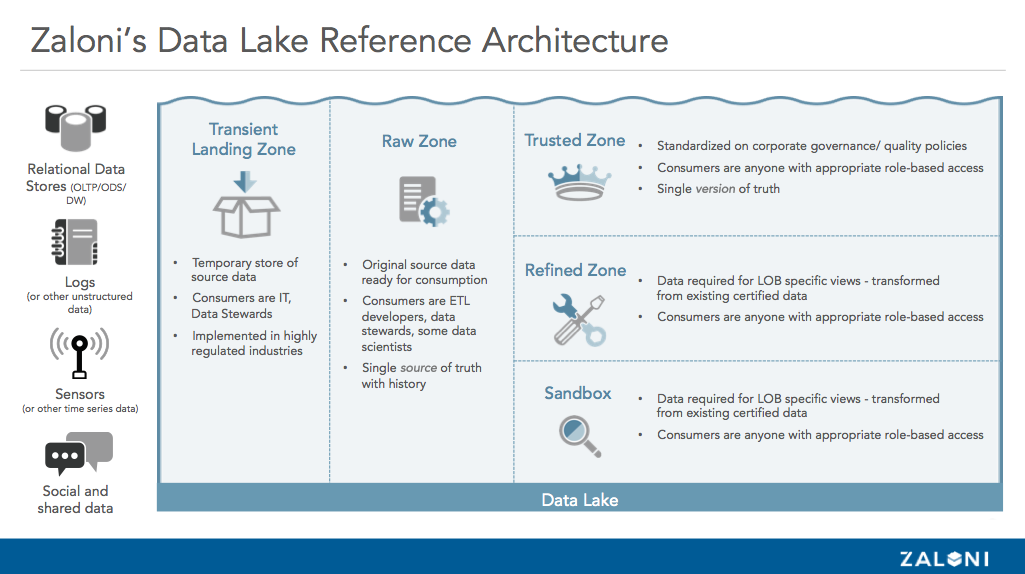
\includegraphics[width=120mm]{data_lake_arch.png}
\caption{\label{data_lake_arch:fig} Typical data lake arch.
}
\end{figure}


\begin{itemize}
\item The data is first loaded into a \textbf{transient loading zone}, where basic data quality checks are performed using MapReduce or Spark by leveraging the Hadoop cluster. 
\item Once the quality checks have been performed, the data is loaded into Hadoop in the \textbf{raw data zone}.

\item An organization can, if desired, perform standard data cleansing and data validation methods and place the data in the \textbf{refined zone}. 

\item From the trusted area, data moves into the \textbf{discovery sandbox}, for wrangling, discovery, and exploratory analysis by users and data scientists.

\item Finally, the consumption \textbf{analytic zone} exists for business analysts, researchers, and data scientists to dip into the data lake to run reports, do "what if" analytics, and otherwise consume the data to come up with business insights for informed decision-making.

\end{itemize}

\begin{center}
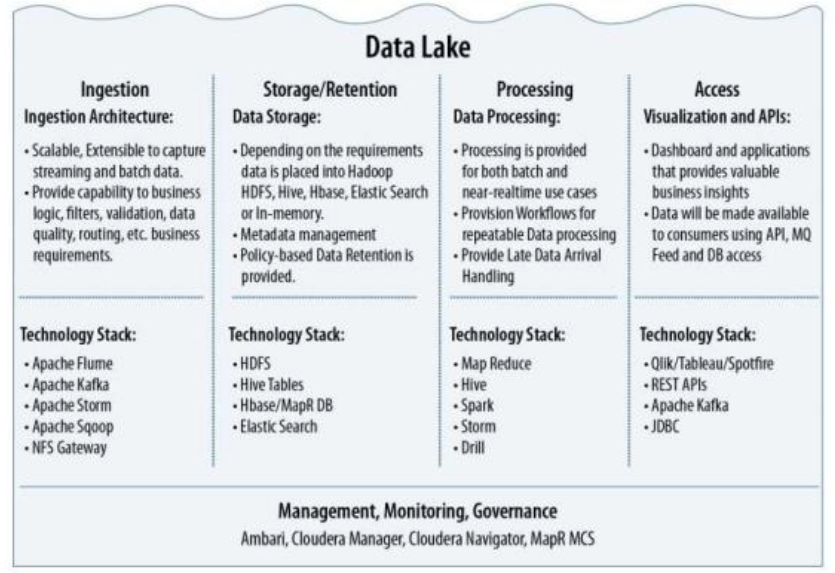
\includegraphics[scale=0.70]{IMAGE10.png}\\
Schema riassuntivo Data Lake
\end{center}

Riassumento, keywords per i data lake sono:

\begin{itemize}[noitemsep]
\item Data Ingestion, ovvero l’acquisizione di dati da fonti esterne che avviene tramite sistemi come Sqoop (RDBMS), Flume (Web Servers), Kafka o Storm (Streaming Data).
\item Storage, basata su un’architettura HDFS.
\item Data Processing, che si suddivide in tre fasi: data preparation, data analystics e result provisioning for consumption. Per effettuare tutte queste operazioni ci si serve di software quali MapReduce, Spark, Flink o Storm. Per eseguire molte attività di manipolazione viene spesso utilizzato NiFi, ovvero un tool workflow based che integra vari applicativi.
\item Data Governance, che comprende Lineage, Integration, Authentication and Authorization, Search, Quality, Audit Logging, Metadata Management, Lifecycle Management e Security.
\end{itemize}
Per acquisire dati in real-time è necessario catturare ogni aspetto di tali dati e con il minimo ritardo possibile. Inoltre, talvolta è necessario sia immagazzinare questi dati in streaming che analizzarli all’istante. La principale limitazione dell’architettura Lambda è che per fare ciò, la logica architetturale va implementata due volte, spesso con tool diversi (Storm, Flink, Spark, …). L’architettura Kappa risolve questo problema.
\section{Data quality and integration}
Fasi molto importanti nell'analisi dei dati sono: la "verifica della qualità dei dati" (Data Understanding), di "pulizia" e di "integrazione" dei dati (Data Preparation).\newline Come primo aspetto, bisogna concentrarsi sui casi di "deduplication"; in altre parole bisogna chiedersi: ci sono record nella stessa tabella che si riferiscono allo stesso oggetto/persona della realtà? Si possono stabilire molteplici regole per decidere se due record si riferiscono allo stesso oggetto, sia sintattiche che semantiche. Una volta individuati due record "analoghi", bisogna unirli (data fusion) in un solo record contenente le informazioni "corrette". Una volta analizzato questo aspetto di "qualità" dei dati, immaginiamoci di dover integrare una tabella con un’altra e quindi di dover cercare i record delle due tabelle diverse che sono collegati tra loro. Questo processo si chiama "record linkage" e può essere svolto, ad esempio, individuando le chiavi delle due tabelle (una primaria e una esterna, ad esempio), e se queste corrispondono si procede con il "merge" dei due record.\newline Tuttavia, se la data quality non è delle migliori (a causa di input sbagliati o di standard non condivisi), di conseguenza anche la data integration sarà scarsa.\newline
La data integration si articola in due fasi: \textbf{record linkage} (identificazione dei set di record che identificano lo stesso "oggetto reale") e \textbf{data fusion} (scelta di un record unico rappresentativo del set precedente).

The complete methodology of schema integration is composed of three possible steps:
\begin{itemize}

\item Schema transformation (or Pre-integration)\\
Input: n source schemas\\
Output: n source schemas homogeneized\\
Methods used: Model transformation + Reverse engineering
\item Correspondences investigation\\
Input: n source schemas\\
Output: n source schemas + correspondences\\
Method used: techniques to discover correspondences (identifying semantic relativism)
\item Schemas integration and mapping generation\\
Input: n source schemas + correspondences\\
Output: integrated schema + mapping rules btw the integrated schema and input source schemas\\
Method used: New classification of conflicts + Conflict resolution
transformations: in particular, type of conflicts are
\begin{itemize}[noitemsep]
\item $Classification\ conflicts$: corresponding elements describe different sets of real world objects\\
Resolution: Introduction of a Generalization/Specialization hierarchy.
\item $Descriptive\ conflicts$: corresponding types have different properties, or corresponding properties are described in different ways.\\
Custom Resolutions depending on the specific type of conflict. %useful, ikr
\item $Structural\ Conflicts$: different schema element types, e.g.: class, attribute, relationship. \\
Resolution: choose the less constraining structure.
\item $Fragmentation\ Conflicts$: the same phenomenon of the real world is perceived as a single S1 object in one database and as several objects in the other\\
Resolution: aggregation relationships.
\item $Instance Level\ Conflicts$: same data in different sources have different
values.
Resolution: user defined $resolution\ function$ (taking two or more conflicting values of an attribute as input and outputs the result to the posed query). Common resolution functions are $MIN$ and $MAX$. For non numerical attributes a typical solution is $CONCAT$.
\end{itemize}
\end{itemize}


\subsection{Record Linkage}
Esistono vari sinonimi per questa fase: Object Identification, Deduplication (su un dataset), Object Matching e molti altri. L’output di un algoritmo di record linkage può essere: "matching tuples", "not matching" o "don’t know" (o "possible matching").\newline
Esistono più tecniche di record linkage:
\begin{itemize}[noitemsep]
\item Empirica, ovvero due tuple vengono unite se la loro distanza (in termini sintattici o anche altre forme di distanza) è piccola.
\item Probabilistica, ovvero una generalizzazione sulla popolazione di regole estratte da un campione.
\item Knowledge Based, ovvero decisioni prese seguendo regole prestabilite.
\item Mixed, ovvero un misto tra il secondo e il terzo approccio.
\end{itemize}
Il record linkage può essere effettuato anche tra set di dati in formati diversi.
%Da valutare se è il caso di aggiungere anche la parte dedicata all'approccio probabilistico.
\subsection{Data Fusion}
Durante questa fase si possono incontrare possibili conflitti.\newline 
Esistono perciò delle strategie per gestire tali conflitti:
\begin{itemize}[noitemsep]
\item $Conflict\ Ignoring$, che ignora il problema lasciando la risoluzione all’utente ($Pass\ It\ on$).
\item $Conflict\ Avoiding$, applica una decisione unica per $tutti$ i dati in conflitto, tipicamente scegliendo una delle fonti come "la più affidabile" e creando il record rappresentativo da quella fonte ($Trust\ Your\ Friends$ strategy).
\item $Conflict\ Resolution$, che fa attenzione a dati e metadati prima di decidere sulla risoluzione del conflitto. Questa strategia può essere divisa in "deciding" (quando viene scelto un valore tra quelli esistenti) e "mediating" (quando viene scelto un valore che non appartiene per forza a quelli esistenti, per esempio la media).
\end{itemize}
\clearpage
\printbibliography
\end{document}
